% !TEX root = ../thesis.tex

% Tässä osassa kuvataan käytetty tutkimusaineisto ja tutkimuksen metodologiset valinnat, sekä kerrotaan tutkimuksen toteutustapa ja käytetyt menetelmät.

% http://en.wikipedia.org/wiki/YUV#Y.27UV420p_.28and_Y.27V12_or_YV12.29_to_RGB888_conversion
% https://msdn.microsoft.com/en-us/library/windows/hardware/ff538197%28v=vs.85%29.aspx

% MITATTAVIA SUUREITA!

\documentclass[thesis.tex]{subfiles}

\begin{document}

\chapter{Design and Implementation}
\label{chapter:design-implementation}

\section{Requirements}

The goal of the thesis was to investigate the feasibility of utilizing smartphone technology to analyze photoluminescent material for product authentication purposes. The example use case was to have a smartphone application that would be able to identify objects (products) tagged with a chemical marker (taggant) as being either fake or authentic. This required implementing a smartphone application that could satisfy the following requirements (requirements \ref{R2} and \ref{R3} refer to the actual product authentication process, whereas \ref{R1} and \ref{R4} are additional feature requirements):

\begin{enumerate}[leftmargin=0.55in, label=\textbf{R\arabic*}]
	\item \label{R1} Support the Windows Phone platform (preferably cross-platform)\\ \\
	Windows Phone was chosen as the initial target platform based on the Lumia 1020 smartphone, which was allocated for the project, and featured one of the best smartphone cameras on the market. An additional goal was set for supporting other major platforms (Android and iOS) in the hopes of being able to compare the results across vendors.

    \item \label{R2} Capture the emission of a luminophore as a function of time\\ \\
    It was outlined that the application should be capable of capturing the emission of a taggant (luminophore) as a sequence of images at pre-defined intervals that should not exceed 1000ms. The sequence of captured images (samples) would work as a unique \emph{fingerprint}. Implementation details, such as the capture method (video vs. images), capture properties (e.g. ISO), or properties of the light source (e.g. wavelength, luminance) were not separately specified.
    % - in relation to Q1

    \item \label{R3} Use the capture data (fingerprint) to query a remote product catalog\\ \\
    The use case (product authentication) required that the fingerprint could be associated with a product. The requirement here was twofold: given a pre-defined database of fingerprints and products associated with them (1) implement a way to use a fingerprint as a query to retrieve a fingerprint corpus and (2) match the fingerprint against the corpus to find the best match to fetch the corresponding product from a remote product database. In case of a match, the user's geolocation should also be stored for further verification and analytics purposes.

	\item \label{R4} Support (secure) offline usage\\ \\
	Implementing support for offline usage was seen as an attractive feature that would differentiate the application from the competition. It would also allow investigating the feasibility of storing data client-side from the perspective of security and storage strategy (size, format).
\end{enumerate}

\noindent The following chapters discuss these requirements further and present the related implementation details. The implementation for \ref{R2} and \ref{R3} is presented in Chapter \ref{chapter:fingerprint-pipeline}. Requirements \ref{R1} and \ref{R4} are discussed in Chapters \ref{chapter:application-architecture} and \ref{chapter:storage-security}, respectively.

\section{Application Architecture}
\label{chapter:application-architecture}

The general architecture of the LuminoTrace application is depicted in Figure \ref{figure:architecture}. The camera application and the external camera module work in tandem to capture and analyze the taggant to construct a fingerprint. To find a product linked to the fingerprint a request is sent over the network to the application server, which queries the databases for a possible match. Alternatively, if the network is unavailable the application will fallback to querying a local copy of the fingerprint database. Finally, the result of the trace is rendered in the UI. In the context of this thesis this process of capturing, analyzing and matching is referred to as \emph{tracing}.

\clearpage

\begin{figure}[h]
\centering 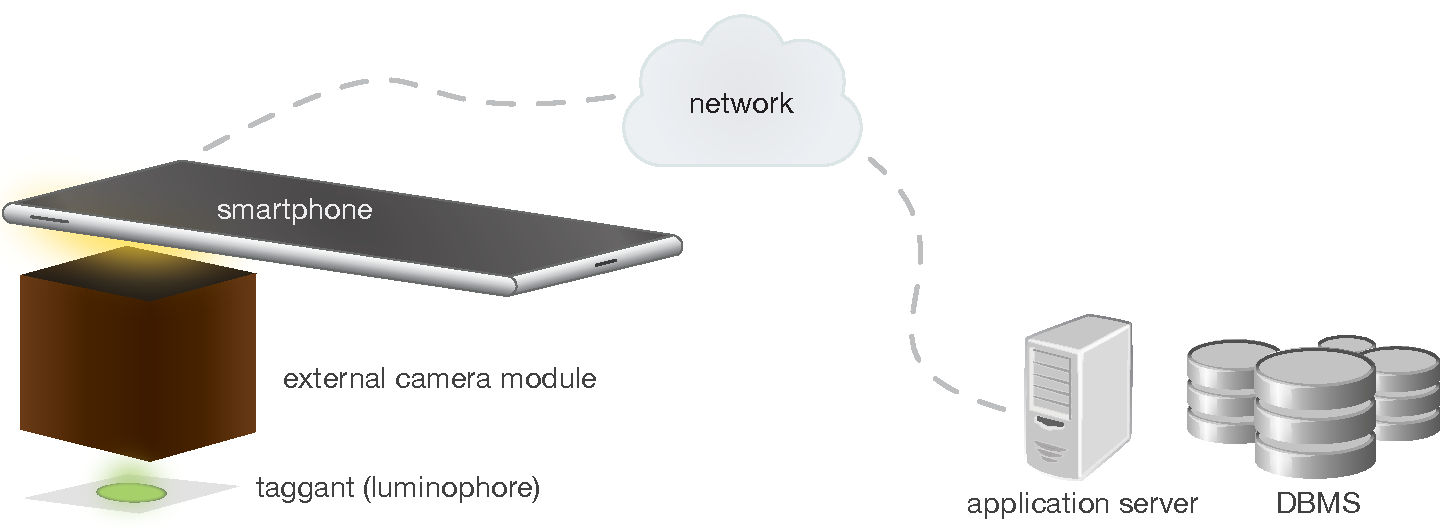
\includegraphics[width=13.5cm]{images/design_implementation/architecture.pdf}
\caption{The general architecture of the LuminoTrace application. The entities involved include a smartphone, an external camera module, a taggant and the cloud (an application server and a DBMS). \label{figure:architecture}}
\end{figure}

\subsection{Camera Application}
\label{chapter:camera-application}

The camera application was implemented as a WebView application using Apache Cordova (4.2.0) and Ionic (1.0.0-beta.14), which allowed supporting multiple platforms with minimal effort as the UI and parts of the application logic could be easily re-used across platforms. Furthermore, no platform-specific knowledge was required to implement the UI allowing focus to be kept on the business logic. Android and Windows Phone were chosen as the target platforms. Support for Android was implemented due to the author's previous experience of the platform and the better debugging tools, which both allowed developing the first prototype faster.

Figure \ref{figure:user_interface} presents the user interface. For brevity, the landing page and the two sidebar views (\emph{Past traces} and \emph{Settings}) are combined into a single image and other views, such as success and error pages, are omitted. The \emph{Past traces} view displays a history of successfully matched products and allows the user to navigate further to view the relevant product information (e.g. product description and link to an online marketplace). The \emph{Settings} sidebar mainly consists of parameters for configuring the underlying algorithms and the smartphone's camera. These settings were only exposed for research and development purposes and would not be displayed to the end-user in the actual application. The main interaction endpoint for the user is the red capture button on the landing page, which initiates the tracing process. The tracing process is discussed in more detail in Chapter \ref{chapter:fingerprint-pipeline}.

\begin{figure}[h]
\centering 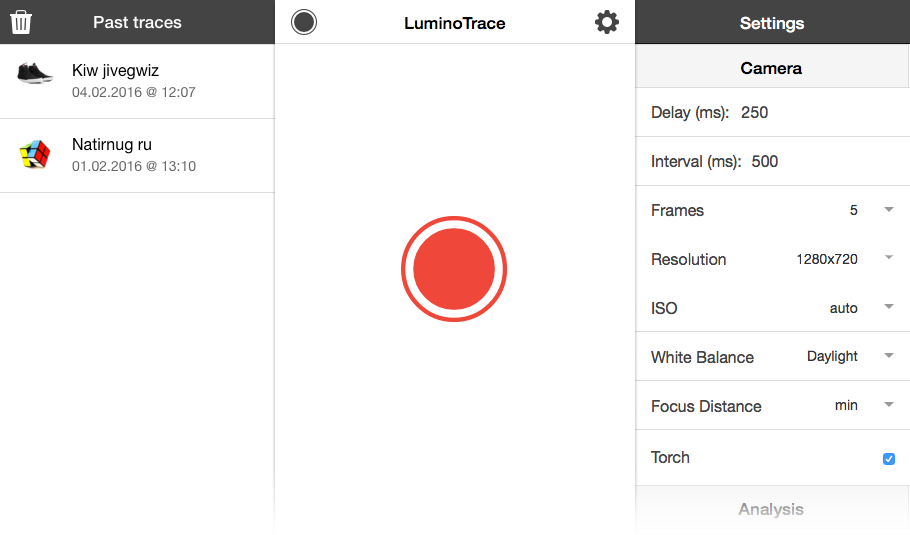
\includegraphics[width=0.83\textwidth,height=\textheight,keepaspectratio=true]{images/design_implementation/user_interface}
\caption{The user interface of the LuminoTrace application consists of two sidebar views for configuring settings and viewing trace history. \label{figure:user_interface}}
\end{figure}

To interact with the native Android and Window Phone camera APIs a custom Cordova plugin was implemented. Existing Cordova camera plugins or native 3rd party camera libraries could not be utilized as a more granular control of the output image data was required. The parameters supported by the plugin and passed to the underlying camera APIs are listed in Table \ref{table:camera-parameters}. Other relevant camera parameters were either disabled (exposure compensation and flash mode) or set to their logical default value (e.g. zoom level of 0). Shutter speed and lens aperture could not be configured due to the lack of support by the API and the hardware, respectively. To capture the fingerprint the plugin interacts with an external camera module. The implementation of the camera module is dicussed in the next chapter.

\begin{table}[ht]
	\caption{Camera parameters supported by the LuminoTrace application.} \label{table:camera-parameters}

	\begin{center}
	\begin{tabular}{| m{2.75cm} | m{9.75cm} |}

		\hline
		\textbf{Parameter}	& \textbf{Description and Supported Values} \\ \hline
		Delay				& Time to wait before starting capture (0-1500ms) \\
		\hline
		Interval 			& Time between subsequent frames (60-1500ms) \\
		\hline
		Frames 				& Number of frames to capture (1-7) \\
		\hline
		Resolution 			& Capture frame resolution (640x480, 1280x720 or max\footnotesize{*}) \\
		\hline
		ISO 				& ISO sensitivity (100, 200, 400, 800, 1600 or auto) \\
		\hline
		White Balance		& White balance preset to use (daylight or auto) \\
		\hline
		Focus Distance		& Distance to which to set the focus to (min or max) \\
		\hline
		Torch 			& Toggle the torch to trigger the camera module (yes/no) \\
		\hline
	\end{tabular}
	\end{center}
	\scriptsize{*} \small{\emph{min} and \emph{max} refer to the minimum/maximum value supported by the platform}
\end{table}

\subsection{Camera Module}
\label{chapter:camera-module}

The camera application is accompanied by an external camera module that consists of a microcontroller, a light source, and a Light-Dependent Resistor (LDR). The purpose of the camera module is to provide a fixed source of light for photoexcitation. The interaction between the camera module and the camera application is "cross-modal": upon capture the camera application toggles the smartphone's torch light, which is detected by the microcontroller using the LDR. The microcontroller in turn triggers the light source, which emits the appropriate wavelength of light to activate the taggant (excite the luminophore). The architecture of the camera module is illustrated in Figure \ref{figure:camera_module}. The camera module encloses the taggant in cardboard to protect it from any ambient light during capture. Pictures of the camera module used in the experiment are included in Appendix \ref{appendix:camera-module}.

\begin{figure}[h]
\centering 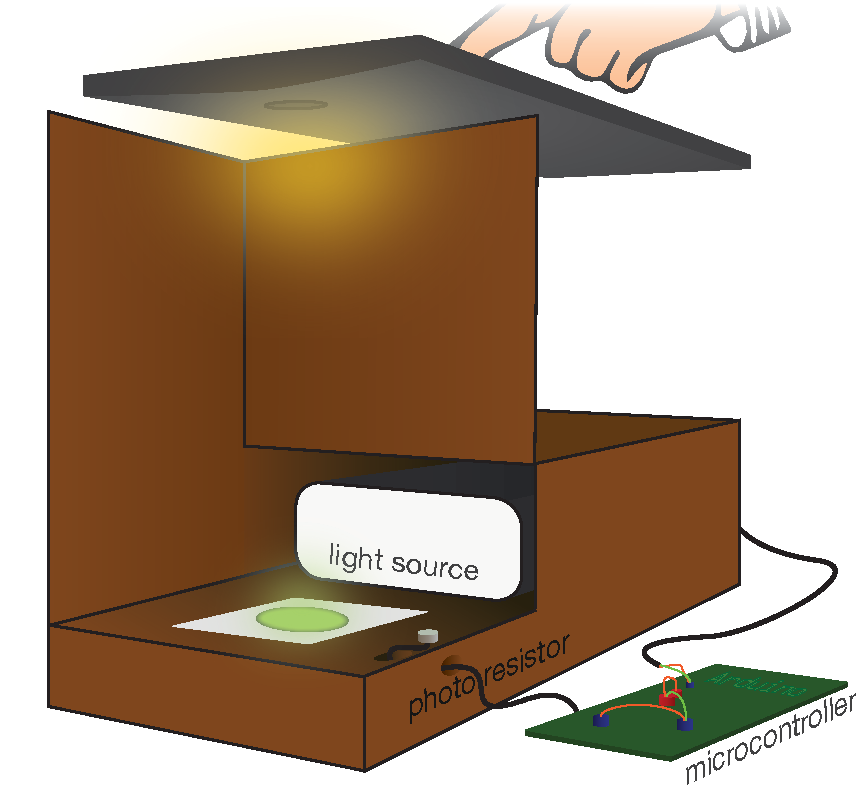
\includegraphics[width=13cm]{images/design_implementation/camera_module.pdf}
\caption{The camera module consists of an external light source, an LDR, and a microcontroller encased in cardboard. \label{figure:camera_module}}
\end{figure}

The architecture of the module embraces modularity to allow easier prototyping. For example, the light source can be detached from the cardboard casing and the microcontroller allowing different kinds of light sources to be used for the photoexcitation. Moreover, the distance between the taggant and the smartphone can be adjusted by switching the detachable cardboard element (highlighted by the dashed line in Figure \ref{figure:camera_module}) to one of different height. This makes it easy to cater for the variety of different minimum focus distances (MFD) smartphone cameras have.

The smartphone's torch light is monitored by a simple program running on the microcontroller. The program reads the resistance of the LDR every 40 milliseconds. The LDR reading changes according to available light: the more light the torch light outputs, the lower is the resistance of the LDR. When a sudden increase in the resistance of the LDR is detected (that is, the torch light has turned off) the microcontroller drives voltage into the circuit causing the light source to be triggered. For added safety the light source is isolated from the rest of the circuit by an optocoupler. The schematics of and the program code running on the microcontroller are included in Appendices \ref{appendix:camera-module-schematics} and \ref{appendix:microcontroller-program}, respectively.

\section{Fingerprint Pipeline}
\label{chapter:fingerprint-pipeline}

The fingerprint pipeline comprises three distinct steps: the capture of the taggant, analysis of the capture data and matching of the resulting fingerprint. A high level overview of the pipeline is provided in Figure \ref{figure:fingerprint-pipeline}. The following subchapters describe these steps in greater detail.

\begin{figure}[h]
\centering 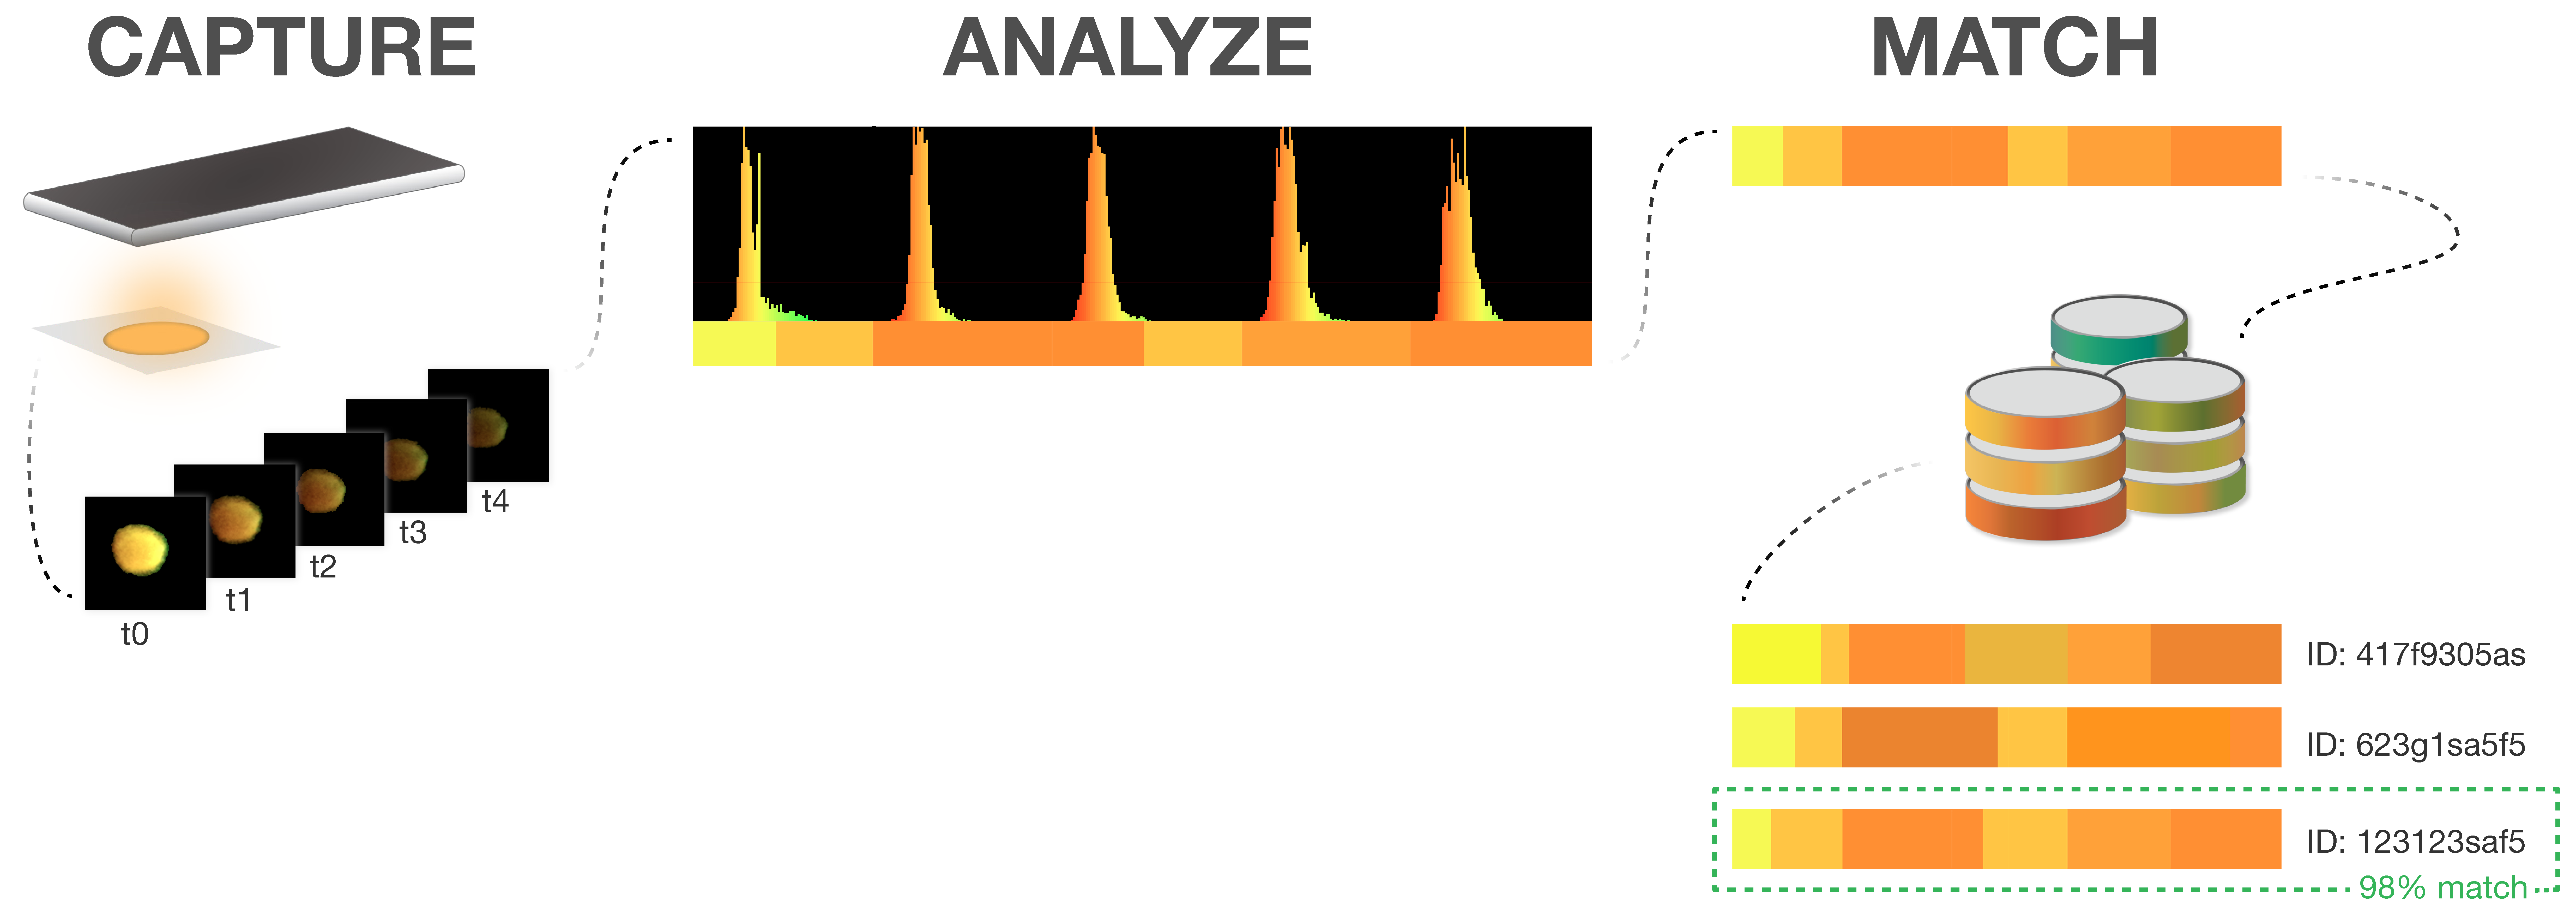
\includegraphics[width=\textwidth,height=\textheight,keepaspectratio=true]{images/design_implementation/fingerprint_pipeline.pdf}
\caption{The fingerprint pipeline consists of capturing a taggant, analyzing it for a fingerprint and finding the best matches. In the context of this thesis the process is referred to as tracing. \label{figure:fingerprint-pipeline}}
\end{figure}

\subsection{Taggant Capture}

The taggant is captured as a sequence of images according to the parameters introduced in Table \ref{table:camera-parameters}. As illustrated in Figure \ref{figure:camera_module} the smartphone is placed on top of the camera module ensuring that the taggant can be isolated from any ambient light, and that the camera will be at the appropriate distance from the taggant -- no closer than the minimum focus distance of the camera. When the user initiates the capture (that is, presses the red capture button as seen in Figure \ref{figure:user_interface}) the camera is first initialized. During initialization the appropriate platform-specific handlers are set and the camera parameters passed via the custom Cordova plugin are applied. After initialization the camera shutter is opened and the torch is toggled to trigger the light source on the camera module. The torch is toggled only after the camera shutter has fully opened to account for any shutter lag.

Once the light source has been triggered the camera application will wait a predefined amount of time (designated by the \emph{delay} parameter in Table \ref{table:camera-parameters}) before capturing the first frame. The duration of the delay is adjusted manually according to the light source: the longer the light decay of the light source, the longer the capture needs to be delayed to avoid artefacts caused by interference. To track the duration of the delay and to schedule the frames to be captured at a given interval a timer is started. As the first frame is ready to be captured the camera application locks the Auto Exposure (AE), Auto Focus (AF) and Auto White Balance (AWB) controls to guarantee that the camera will use the same exposure, focus and white balance settings for the subsequent frames. Finally, each captured frame is sent to an analyzer component for further processing. The taggant capture process is summarized in Figure \ref{figure:taggant-capture-process}.

\begin{figure}[h]
\centering 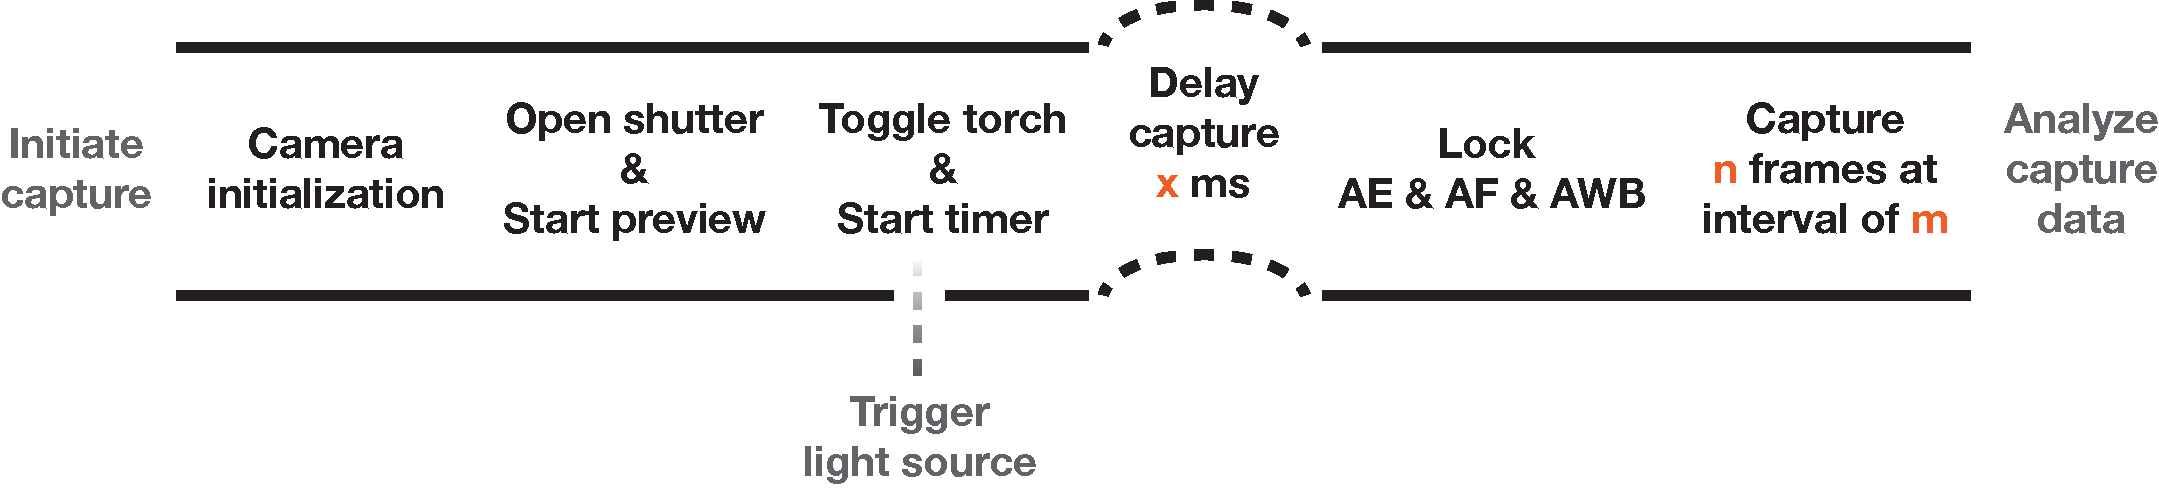
\includegraphics[width=\textwidth,height=\textheight,keepaspectratio=true]{images/design_implementation/capture_process.pdf}
\caption{The taggant capture process. \label{figure:taggant-capture-process}}
\end{figure}

The image sequence is not captured as individual frames, but instead, due to the lack of proper support by the respective camera APIs, data is captured from the camera's preview feed. The output from the sensor is read in the YCbCr format. Android encodes the data in the NV21 format whereas Windows Phone uses the NV12 format. The difference between NV21 and NV12 is that the interleaving order of the Cr and Cb samples is the opposite. The subsampling ratio of these formats is 4:2:0. The rate at which new preview frames are capture depends on the Frames Per Second (FPS) supported by the sensor. Higher rate of frames allows shorter intervals to be used, and thus, the preview FPS is set to the highest possible value (or, range) supported by the platform during the camera initialization.

\subsection{Taggant Analysis}

The purpose of the taggant analysis step is to construct a unique fingerprint from the captured frames. The analysis process is outlined in Figure \ref{figure:taggant-analysis-process}. To prevent blocking the main UI thread and affecting the capture performance the frames are processed (analysed) concurrently in their own threads.

\begin{figure}[h]
\centering 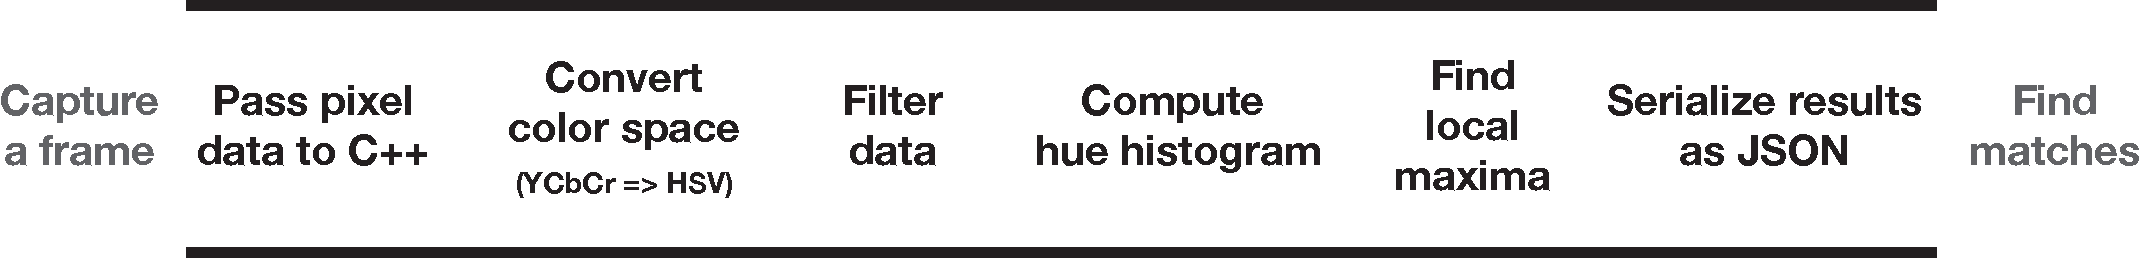
\includegraphics[width=\textwidth,height=\textheight,keepaspectratio=true]{images/design_implementation/analysis_process.pdf}
\caption{The taggant analysis process; frames are processed concurrently in separate threads to avoid blocking the UI.\label{figure:taggant-analysis-process}}
\end{figure}

Each frame is processed using C++ so that the functionality can be easily reused across platforms. On Android and Windows Phone, calls between the native code and the C/C++ libraries are marshalled using the Java Native Interface (JNI) and the C++/CX component extensions, respectively. Another benefit of moving the frame processing to be done in C++ is the number of robust libraries available for signal processing. The analysis algorithm utilizes the OpenCV\footnote{\url{http://opencv.org/}} open source computer vision library (version 2.4.9) for most of its computations.

The analysis algorithm uses the hue histogram of a captured frame as the basis for the analysis. For each frame the algorithm finds the most dominant hues (hue peaks). The array of peaks computed from the all the frames form a unique \emph{fingerprint}. The process consists of multiple processing steps. Each frame first goes through a color space conversion, where the pixel data is converted from the native YCbCr format to RGB, and then to HSV as per Equation \ref{rgb-to-hsv} utilizing OpenCV's color conversion API. The data is then filtered for noise using binary thresholding, which uses the frame's grayscale information (V channel) to filter pixels that fall outside a certain intensity level (brightness threshold). The thresholding process is illustrated in Figure \ref{figure:binary-thresholding}.

\begin{figure}[h]
\centering 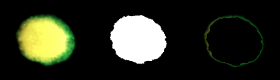
\includegraphics[width=\textwidth,height=\textheight,keepaspectratio=true]{images/design_implementation/binary_thresholding}
\caption{The algorithm uses binary thresholding for noise reduction. The original frame is on the left and the threshold mask is in the middle. The image on the right shows the pixels that would fall outside the threshold.\label{figure:binary-thresholding}}
\end{figure}

The hue histogram can be computed from the filtered HSV data using OpenCV's \emph{calcHist()} function with an appropriate bin size for the hues (1-180). The hue peaks are computed from the normalized hue histogram using an open source library called Persistence1D \cite{persistence1d}. Persistence1D selects the peaks (local maxima) based on a persistence threshold (0-1), which denotes the minimum required delta between a local maxima and minima pair. For example, a persistance threshold of 0.20 would mean that a local minima/maxima pair would only be formed if the delta between the two points were greater than 20\%. Each peak is stored as a 2D point: $P(hue, intensity)$.

Once all the frames have been captured and their peaks have been computed a fingerprint can be constructed. Given a sequence of \emph{n} frames and a number \emph{m} denoting the most peaks found for a single frame (sample) in the sequence the fingerprint can be described as a $n \times m$ matrix. The algorithm encodes the matrix as a JavaScript array and augments it with useful metadata (e.g the capture timestamp of each frame) before sending it to the fingerprint matching algorithm for further processing. An example of the fingerprint output format is provided in Appendix \ref{appendix:fingerprint}.

\subsection{Fingerprint Matching}
\label{chapter:fingerprint-matching}

In the fingerprint matching step the fingerprint is matched against an existing set of fingerprints (corpus) to find the best match. The query for fetching the relevant corpus is constructed based on the peak count and average hue of the fingerprint's first sample (the first row of the $n \times m$ fingerprint matrix as per Appendix \ref{appendix:fingerprint}). The average hue is calculated as a weighted arithmetic mean using the hue intensities as the weights. To allow more flexible queries the value for the peak count and average hue can also be provided as a range. The query format and the databases involded are discussed in more detail in Chapter \ref{chapter:storage-security}.

The fingerprint and the retrieved corpus are given as input to a matching algorithm implemented in JavaScript. The algortihm ranks the captured fingerprint (subject fingerprint) against the fingerprints in the corpus (candidate fingerprints) based on two simple metrics:

\begin{itemize}
	\item Peak Hue Delta ($P_{hue}$): the difference in peak hue
	\item Peak Intensity Delta ($P_{int}$): the difference in peak hue intensity
\end{itemize}

The subject fingerprint and a candidate fingerprint are compared sample by sample (frame by frame). That is, the deltas are computed between each $n$th sample of the two fingerprints. The metrics $P_{hue}$ and $P_{int}$ are given different weights and thresholds. $P_{hue}$ is given more weight and a lower threshold as fingerprints that have dissimilar dominant hues are not likely to be a good match. $P_{int}$ is given a smaller weight and a higher threshold since slight variations in hue intensities are expected due to noise in the pipeline. The formula used for computing the similarity metrics for a fingerprint is given as follows:

\begin{equation}
\label{equation:similarity-metric}
	P_x = \sum \limits_{n=0} \sum \limits_{i=0} { { w_x \cdot \max (\Delta{x_i}-t_x,\ 0) \cdot d_x^n } }
\end{equation}

Where:
\begin{itemize}[label=]
	\setlength\itemsep{0.10em}
    \item $P_x$: metric for dimension $x$ (e.g. $P_{hue}$)
    \item $n$: sample of the fingerprint
    \item $i$: peak in the sample
    \item $w_x$: weight for dimension $x$
    \item $\Delta{x_i}$: delta in dimension $x$ between peak $i$ and its pair
    \item $t_x$: delta threshold for dimension $x$
    \item $d_x$: damping coefficient for dimension $x$
\end{itemize}

\noindent The purpose of the damping coefficient $d_x$ ($\leq 1$) is to put less emphasis on the latter samples of the fingerprint as it is expected that the first samples are more descriptive of the entire fingerprint (include less noise). The metric $P_x$ is \emph{monotonically increasing} meaning that the larger its value, the more dissimilar the fingerprints (hence also the notation $P$ as in penalty).

In order to compute $P_x$ (or, more specifically $\Delta{x_i}$) the peaks of the subject and candidate fingerprints have to be paired with each other. The pairing of the peaks can be expressed as an \emph{assignment problem} where each peak in sample $A_n$ of fingerprint $A$ needs to be paired with a peak in sample $B_n$ of fingerprint $B$ with minimal cost (change in hue). An algorithm suitable for solving the assignment problem for small datasets is the Hungarian algorithm \cite{hungarian_algorithm}, which takes an $n \times m$ \emph{cost matrix} as input and outputs a $min (n,\ m)$ number of $(i, j)$ coordinates (pairs) that represent the minimum cost.

Each cell $a_{ij}$ of the cost matrix $C$ represents the hue delta between the $i$th peak of $B_n$ and $j$th peak of $A_n$. Thus, the dimensions of the matrix are given by the number of peaks in $A_n$ and $B_n$. The cost matrix and the pairings computed by the algorithm are illustrated in Figure \ref{figure:hungarian-algorithm}.

\begin{figure}[h]
\centering 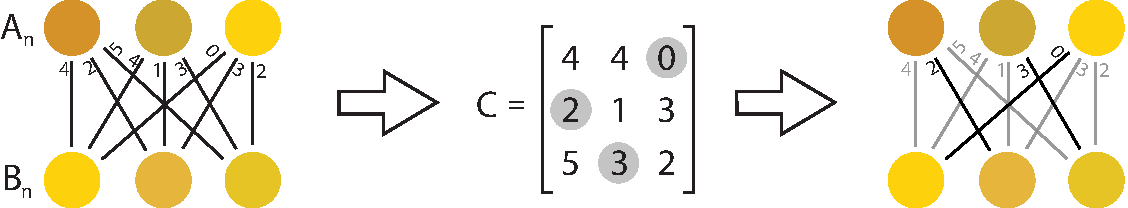
\includegraphics[width=\textwidth,height=\textheight,keepaspectratio=true]{images/design_implementation/hungarian_algorithm}
\caption{The Hungarian algorithm is used in the fingerprint matching process to find the lowest-cost way to pair peaks of two fingerprint samples. $A_n$ and $B_n$ denote the samples, for which the cost matrix $C$ is computed.\label{figure:hungarian-algorithm}}
\end{figure}

The Hungarian algorithm does not, however, provide a solution for the \emph{unbalanced assignment problem}: non-square cost matrices ($n \neq m$) are always left with unpaired rows/columns as the algorithm only returns $min (n,\ m)$ number of pairs. This becomes an issue in cases where samples $A_n$ and $B_n$ have a different number of peaks. To overcome this limitation the matching algorithm extends the Hungarian algorithm by finding the lowest-cost pair for any unpaired rows/columns (peaks). The logic of the extended functionality supporting non-square cost matrices is illustrated in Figure \ref{figure:hungarian-algorithm-extended}.

\begin{figure}[h]
\centering 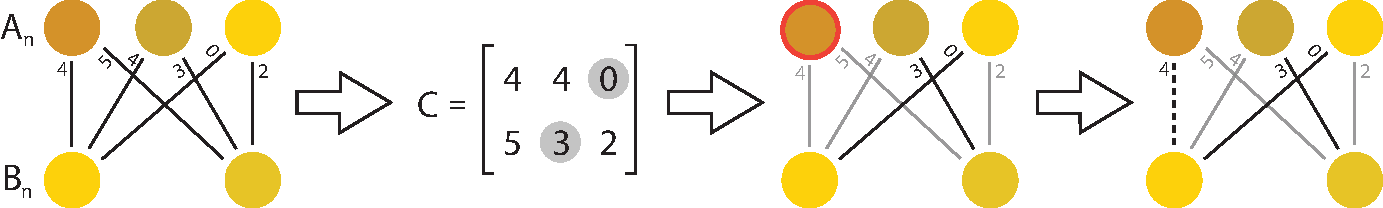
\includegraphics[width=\textwidth,height=\textheight,keepaspectratio=true]{images/design_implementation/hungarian_algorithm_ext}
\caption{The functionality of the Hungarian algorithm is extended by a custom implementation to handle non-square cost matrices.\label{figure:hungarian-algorithm-extended}}
\end{figure}

\noindent The Hungarian algorithm used by the similarity matching algorithm is based on a 3rd party JavaScript implementation \cite{munkres-js}.

To account for an edge case where a (subject/candidate) fingerprint sample $n$ includes no peaks -- and thus, no peak pairs would be found to compute $P_{hue}$ and $P_{int}$ for that sample -- an additional penalty metric $P_c$ is applied:

\begin{equation}
\label{equation:similarity-metric-no-peaks}
P_c = \sum \limits_{n=0} { w_c \cdot \Delta{c_n} \cdot d_c^n }, \qquad
\Delta{c_n} = \begin{cases}
|a_n - b_n| &\text{if $a_n \cdot b_n = 0$}\\
0 &\text{otherwise}
\end{cases}
\end{equation}

Where:
\begin{itemize}[label=]
	\setlength\itemsep{0.10em}
    \item $n$: sample of the fingerprint
    \item $w_c$: weight for peak count delta
    \item $\Delta{c_n}$: peak count delta between fingerprints $a$ and $b$ for sample $n$
    \item $d_c$: damping coefficient for peak count delta
\end{itemize}

\noindent Given Equation \ref{equation:similarity-metric} for metrics $P_{hue}$ and $P_{int}$ and Equation \ref{equation:similarity-metric-no-peaks} for the additional penalty metric $P_c$ the total penalty $P$ for a candidate fingerprint can be expressed as follows:

\begin{equation}
	P = P_{hue} + P_{int} + P_{c}
\end{equation}
\\
Once the candidate fingerprints have been ranked the best matches are selected based on two boundary conditions: the top four candidates that are within a 75\% margin of the best candidate qualify. The values for the boundary conditions are derived from the experiment data presented in Chapter \ref{chapter:results}.

If the algorithm finds a matching fingerprint the application fetches the user the corresponding product for display. In case multiple matches are found and the result of the matching process is therefore \emph{inconclusive}, the user is displayed a list of products and asked to verify whether or not it includes the traced product -- if not, the product is deemed fake. Links between fingerprints and products are stored in and retrieved from a database. The storage architecture and related security is discussed in the next chapter. The fingerprint matching process is summarized in Figure \ref{figure:matching-process}.

\begin{figure}[h]
\centering 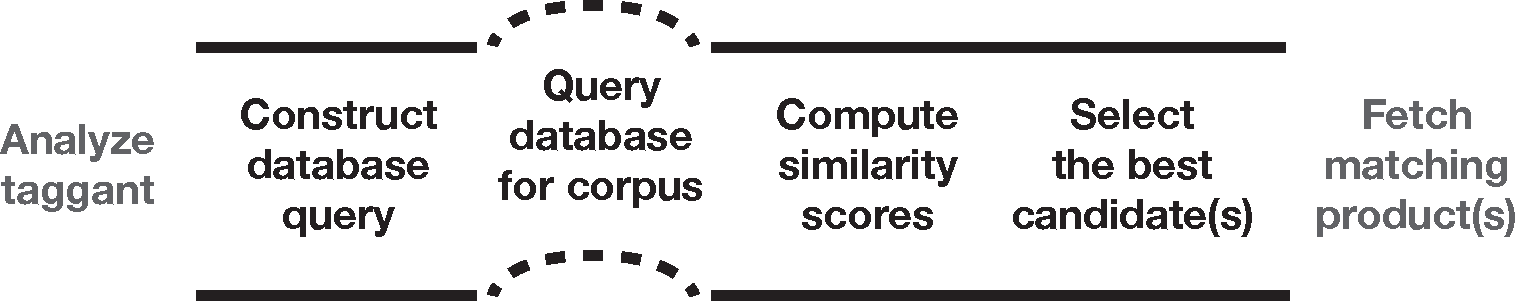
\includegraphics[width=0.9\textwidth,height=\textheight,keepaspectratio=true]{images/design_implementation/matching_process}
\caption{The fingerprint matching process.\label{figure:matching-process}}
\end{figure}

\section{Application Storage and Security}
\label{chapter:storage-security}

The application is backed by an application server and a remote Database Management System (DBMS). The application fetches data both directly through the DBMS as well as via the application server. Data is also persisted on the device to enable offline usage. The DBMS is implemented using a NoSQL database technology called CouchDB\footnote{\url{http://couchdb.apache.org/}} (version 1.6.1) while the application server runs on Node.js\footnote{\url{http://nodejs.org/en/}} (version 5.5.0). For the local device storage the application utilizes PouchDB\footnote{\url{http://pouchdb.com/}} (3.2.0) and Mozilla's localForage\footnote{\url{http://mozilla.github.io/localForage/}} (version 1.2.0) browser libraries, which wrap the browser's (web view's) storage APIs (IndexedDB, WebSQL and localStorage) in a more stable, asynchronous API.

The fingerprint corpus, products and the mappings between them as well as metadata about the capture configurations (ISO, delay...) and the taggants are persisted by the DBMS (a CouchDB instance). Each document in the products database consists of minimal product information (title, description, brand name...) and IDs that could -- in an actual business scenario -- be used as a reference to an item in a brand's internal product management system. The mapping information linking fingerprints to products is stored in a separate fingerprint metadata database. For brevity, the schema of a fingerprint metadata document is presented in Table \ref{table:fingerprint-metadata-schema}.

\begin{table}[ht]
	\caption{The structure of a fingerprint metadata document.} \label{table:fingerprint-metadata-schema}

	\begin{center}
	\begin{tabular}{| m{1.25cm} | m{11.5cm} |}

		\hline
		\textbf{Key}	& \textbf{Description} \\ \hline
		\_id			& The unique ID of the metadata document assigned by CouchDB \\
		\hline
		\_rev 			& Document hash used by the CouchDB replicator to track changes \\
		\hline
		fid 			& ID of the fingerprint the metadata describes \\
		\hline
		pid 			& ID of the product the fingerprint is linked to \\
		\hline
		cid 			& ID of the configuration the fingerprint was captured with \\
		\hline
		tid 			& ID of the taggant the fingerprint is based on \\
		\hline
		created			& Timestamp to denote when the fingerprint was created \\
		\hline
	\end{tabular}
	\end{center}
\end{table}

\noindent The IDs \emph{cid} and \emph{tid}, and the created timestamp are unique together. They convey the information of when and how a specific taggant was analyzed for fingerprints.

The application interacts with the application server and the DBMS during application initialization and the fingerprint matching process. When the application is launched the user is automatically logged in to the DBMS using a predefined username and password. The authentication can be performed directly against the DBMS as CouchDB provides a built-in authentication framework through a RESTful interface. However, as the application and the DBMS communicate via XHR but live in different domains, CORS needs to be enabled on the DBMS to allow cross-domain requests. Both the application server and the DBMS run over TLS to protect them from man-in-the-middle (MitM) attacks.

Once the user has been successfully authenticated with the DBMS the fingerprints are synced to the user's device for offline use. The syncing functionality is implemented using PouchDB, which supports replication and synchronization of CouchDB databases into the browser utilizing CouchDB's revisioning features (the detailed description of the replication mechanisms between PouchDB and CouchDB is outside the scope of this thesis and the reader is thereby advised to refer to \cite{pouch-couch-replication} for further information). In the browser, the data is persisted by PouchDB using one of supported persistence backends (IndexedDB, WebSQL or localStorage). Persisting the fingerprints and the fingerprint metadata in different databases allows the fingerprints to be synced independently of the metadata. This has both performance and security implications as it ensures that only the minimum required data is synced to the user's device for offline use, and that no additional information about the fingerprint (e.g. capture conditions) is exposed to malicious parties.

During the fingerprint matching process the fingerprint database is queried for a corpus -- either over network or locally depending on network availability. As discussed earlier in Chapter \ref{chapter:fingerprint-matching}, the query is specified in terms of peak count and weighted hue average of the fingerprint's first sample ($n=0$). Moreover, the values for the query can be provided as a range. To allow fingerprints to be queried this way directly a separate view of the data -- an index keyed by the peak count and the weighted hue average of the first sample -- needs to be constructed. With CouchDB this can be achieved using a \emph{design document}, which allows documents in a database to be map-reduced into a separate view. The custom design document used by the CouchDB instance to construct a new fingerprint view (named \emph{find\_by\_peak\_count}) is provided in Appendix \ref{appendix:fingerprint-design-doc} for reference.

When the remote fingerprint database is queried over the network the parameters for the fingerprint query are provided in the request URL's query parameters. For example, a query to fetch a fingerprint corpus that consists of fingerprints whose first sample's peak count and weighted hue average range from 3 to 5 and 68 to 78, respectively, is formatted as follows (the beginning of the request URL is omitted for brevity):\\

% \begin{itemize}[label=]
\colorbox{gray!10} {\quad \small .../\_view/find\_by\_peak\_count\_and\_hue?startkey=[3,68]\&endkey\=[5,78] \quad} \\
% \end{itemize}


\noindent PouchDB also appends a pseudo-random number (\emph{nonce}) to the query string to protect the client from replay attacks.

If the retrieved corpus includes a match, the ID of the matched fingerprint (\emph{fid}) is sent to the application server to fetch the corresponding product. The application server uses the \emph{fid} to query the fingerprint metadata database for the associated product ID (\emph{pid}), which it then uses to retrieve the correct product from the products database. The product information of a successfully matched fingerprint is persisted locally as \emph{trace history} using localForage. If the application server is unavailable or the user is offline when a product is queried for, the application displays a dummy product and schedules the product information to be synced when the application is launched the next time.

Figure \ref{figure:application-database-flow} provides a summary of the storage architecture and the communication scenarios between the application, the application server and the DBMS.

\enlargethispage{10\baselineskip}

\begin{figure}[h]
\centering 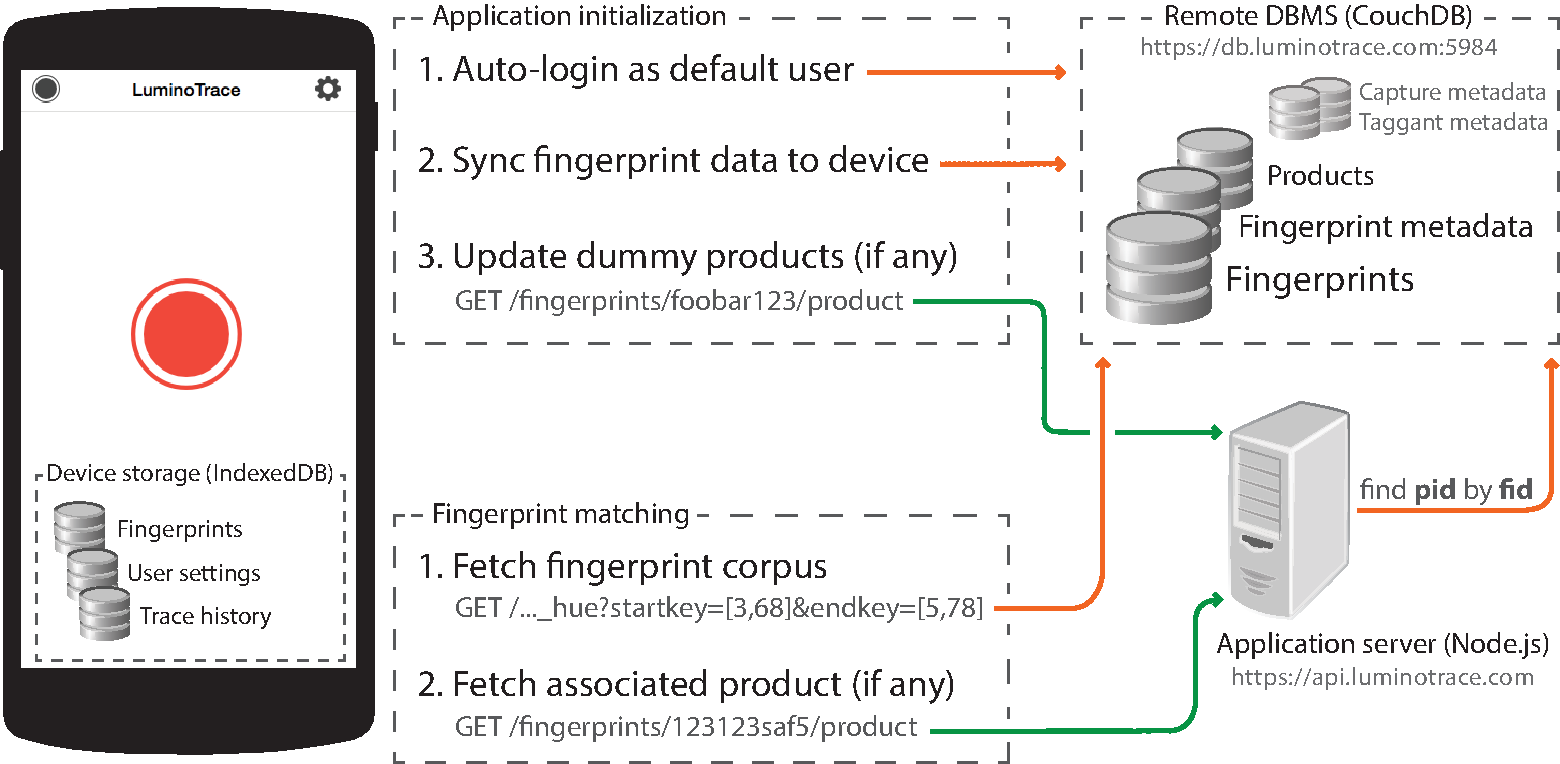
\includegraphics[width=\textwidth,height=\textheight,keepaspectratio=true]{images/design_implementation/application_database_flow}
\caption{The application interacts with a Node.js application server and a RESTful CouchDB instance during application initialization and the fingerprint matching process. Fingerprints are synced to the device storage for offline usage.\label{figure:application-database-flow}}
\end{figure}

\end{document}